\subsection{Planificación temporal}\label{sec:planning}
El proyecto, dio comienzo en octubre del 2014 y finalizará en abril de 2015, por tanto tendrá una duración estimada de siete meses. Se ha establecido que los \textit{sprints} tendrán una duración aproximada de cuatro semanas, con lo cual toda la planificación va guiada a hacer tareas concretas dentro de ese lapso de tiempo. 

La dedicación al proyecto sera de treinta horas semanales, seis horas por dia laborable, a los cuales hay que restar una semana de vacaciones de navidad. \\
Por tanto: 
\begin{eqnarray} 
(30 \mbox{ horas/semana } \cdot 4 \mbox{ semanas/mes}) \cdot  7 \mbox{ meses }) - (6 \mbox{ horas}\cdot 5\mbox{ dias}) = 810 \mbox{ horas}
\end{eqnarray}
Con lo cual se dedicarán \textit{810 horas} a la realización del proyecto, las cuales se dividirán de acuerdo a la planificación que se muestra en el diagrama de Gannt de la figura \ref{fig:diagrama_gantt}:

\begin{figure}[ht]
    \centering
    \includegraphics*[scale=0.75]{GEP/planning/tablaPlanning.png}
\end{figure}

\begin{figure}[ht]
    \centering
    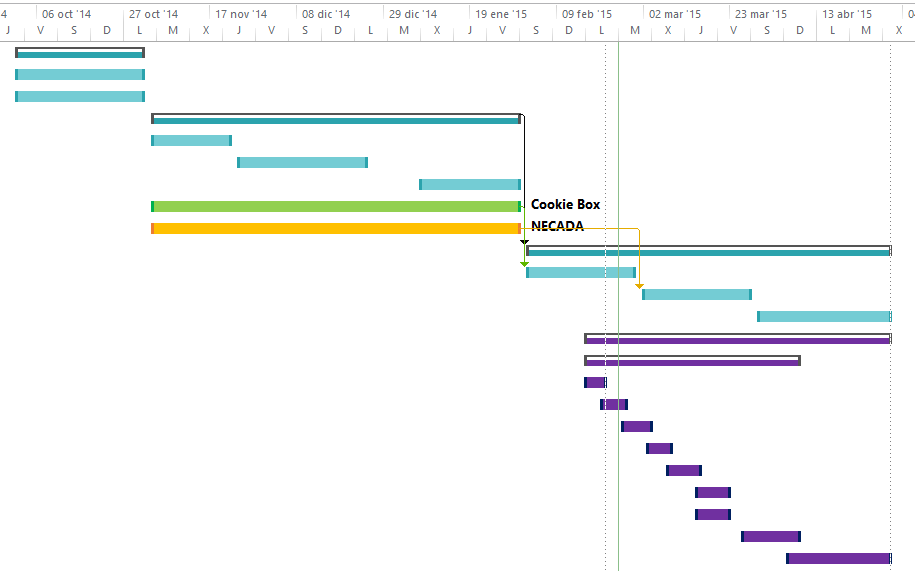
\includegraphics[width=1.0\linewidth]{GEP/planning/gannt.PNG}
    \caption[Diagrama de Gannt]{Diagrama de Gannt}
    \label{fig:diagrama_gantt}
\end{figure}
\FloatBarrier

En el diagrama se ha representado en azul las fases y tareas correspondientes a investigación y desarrollo por parte del equipo y en morado las tareas correspondientes a documentación del proyecto. El resto de colores simbolizan tareas que son necesarias para el proyecto, pero no son responsabilidad del equipo de desarrollo.

Como ya se ha comentado para la validación de las tareas se utilizarán las reuniones al final de cada \textit{sprint}, con lo cual las fases contarán con uno o dos \textit{sprints} dependiendo de la duración de estas.

\subsubsection{Definición de tareas}

\begin{description}
  \item[Fase 1] Preparación previa\\
  El primer mes del proyecto se dedicará a la preparación previa de este.
    \begin{itemize}
        \item \textbf{Tarea 1.1} Definición del sistema\\
        Durante esta fase, se definirán cuales son las necesidades del proyecto, objetivos y funcionalidades que se espera que este incorpore.
        
        Una vez definidas las necesidades, se estudiarán las distintas alternativas posibles para integrar el proyecto dentro del sistema.
        \item \textbf{Tarea 1.2} Estudio nuevas tecnologías\\
        En paralelo con la definición del sistema se realizará un estudio de la tecnologia que se escoja para la realización del proyecto. Es decir, al tratarse de una tecnologia desconocida esta requiere un tiempo de aprendizaje para poder realizar el proyecto de forma correcta.
    \end{itemize}
  \item[Fase 2] Desarrollo básico\\
  Una vez decidida la tecnologia a utilizar y asimilados los conceptos básicos para poder dar comienzo, se desarrollará el primer prototipo del proyecto.
    \begin{itemize}
        \item \textbf{Tarea 2.1} Configuración del entorno\\
        Para empezar a desarrollar el proyecto, lo primero que se realizará será una configuración del entorno, la cual consisitirá en preparar un repositorio para el control de versiones del proyecto y configurar toda la estructura del portal web.
        \item \textbf{Tarea 2.2} Gestión de usuarios\\
        La primera funcionalidad que se desarrollará del portal será la gestión de usuarios, dentro de esta tarea se espera que un usuario sea capaz de registrarse en el portal (con un nombre de usuario y contraseña) y posteriormente ingresar en él.
        \item \textbf{Tarea 2.3} Gestión de hogares I (como usuario \textit{Empresa})\\
        En este punto se desarrollará una parte de la gestión de hogares, la que entendemos que utilizaran los usuarios nombrados como \textit{Empresa}. Los puntos que se realizarán en esta tarea será la posibilidad de crear un inmueble y editarlo.
        \item \textbf{Tarea 2.4} Definición de la gamificación (\textit{COOKIEBOX})\\
        De forma paralela al desarrollo del primer prototipo, \textit{COOKIEBOX} se encargará de la definición de la gamificación que posteriormente se utilizará en el portal. La gestión de hogares II dependerá directamente de la definición de la gamificación.
        \item \textbf{Tarea 2.5} Obtener datos simulación (\textit{NECADA})\\
        \textit{NECADA} se encargará de realizar en paralelo una serie de simulaciones para obtener los datos necesarios para el sistema, pese a no ocuparnos de forma directa de esta tarea es importante tenerla en cuenta ya que hasta no tener el resultado de las simulaciones no será posible empezar con la gestión de hogares II. 
    \end{itemize}
  \item[Fase 3] Desarrollo avanzado\\
  Una vez desarrollado el primer prototipo se pasará al desarrollo del resto de funcionalidades del proyecto.
  \begin{itemize}
        \item \textbf{Tarea 3.2} Desarrollo de la gamificación\\
        Una vez definida la gamificación esta se implantará en el portal web, siguiendo las directrices dadas por \textit{COOKIEBOX}. 
        \item \textbf{Tarea 3.3} Gestión de hogares II (como usuario \textit{Particular})\\
        El usuario \textit{Particular} ha de ser capaz de crear hogares y editarlos. En este punto, se espera que la cantidad de información que aporte un \textit{Particular} sea mucho mayor que la de la empresa, con esta información se le mostrará al usuario sus datos de consumo (obtenidos de \textit{NECADA}).
        \item \textbf{Tarea 3.4} Sistema de recomendaciones\\
        Una vez un usuario \textit{Particular} haya dado los datos de su hogar, el sistema le indicará distintas maneras de optimizar el consumo de este. Un ejemplo de recomendación sería el caso de un usuario que utiliza bombillas de bajo consumo, el sistema le recomendará que las cambie a LED, dándole información aproximada del ahorro y la inversion que esto le conllevaria.
    \end{itemize}
  \item[Fase 4] Desarrollo memoria\\
  Se ha decidido crear una fase diferenciada para la creación de la memoria, esta fase dará comienzo junto con la asignatura de GEP y a partir de entonces, el desarrollo de esta será paralelo con el proyecto.
    \begin{itemize}
        \item \textbf{Tarea 4.1} GEP\\
        Las distintas tareas que se encuentran aquí son las entregas relacionadas con la asignatura de GEP y las presentaciones que se realizan dentro de esta.
         \begin{itemize}
            \item \textbf{Tarea 4.1.1} Alcance del proyecto
            \item \textbf{Tarea 4.1.2} Planificación temporal
            \item \textbf{Tarea 4.1.3} Gestión economica y sostenibilidad
            \item \textbf{Tarea 4.1.4} Presentación preliminar
            \item \textbf{Tarea 4.1.5} Contextualizacion y bibliografia
            \item \textbf{Tarea 4.1.6} Pliegue de condiciones
            \item \textbf{Tarea 4.1.7} Entrega presentación oral y documento final
            \item \textbf{Tarea 4.1.8} Presentación oral
         \end{itemize}
        \item \textbf{Tarea 4.2} Realizar el resto de documentación\\
        Una vez finalizado GEP se procederá a la realización del resto de la memoria.
    \end{itemize}
\end{description}

\subsubsection{Valoración de alternativas y planes de acción}
Al tratarse de un proyecto que utiliza metodologías ágiles, las posibles desviaciones que se vayan produciendo en este serán corregidas en las reuniones que se realizan al final de cada \textit{sprint}.

Con esto se consigue que si en cualquier momento se encontrará alguna desviación demasiado grande en la planificación prevista del proyecto se aplicarían un seguido de medidas correctivas, así como buscar cual ha sido el problema de esta desviación. Dentro de estos \textit{sprints} también se definirán de forma concreta las tareas a realizar, con lo cual si se viera que no es posible llegar a las fechas acordadas se buscaría una solución que pueda satisfacer al cliente y a su vez entre dentro de la planificación.

Dentro de este proyecto contamos con dos casos que pueden suponer un retraso al proyecto muy importante, estos son la \textbf{Tarea 2.4} Definición de la gamificación y la \textbf{Tarea 2.5} Obtener datos simulación ya que son tareas que dependen de terceros y para la realización de algunas tareas es imprescindible que estén finalizadas.

Si se diera el caso que estas tareas no estuvieran realizadas dentro del tiempo establecido en la planificación se procedería a realizar otras tareas las cuales no cuenten con ninguna dependencia o incluso se podría llegar a trabajar de forma paralela, es decir, realizar la \textbf{Tarea 3.2} Desarrollo de la gamificación a la vez que se recibe la definición de la gamificación de la empresa \textit{COOKIEBOX} y de la misma manera con la \textbf{Tarea 3.3} Gestión de hogares II.

\subsubsection{Recursos}

\begin{table}[h]
\begin{center}
\begin{tabular}{@{}cc@{}}
\toprule
\textbf{Recurso Hardware} & \textbf{Funcionalidad} \\ \midrule
Ordenador & Necesario para el desarrollo del proyecto \\ \bottomrule
\end{tabular}
\end{center}
\caption{Recursos hardware del proyecto. \label{tab:recursosHard}}
\end{table}

\begin{table}[h]
\begin{center}
\begin{tabular}{@{}cc@{}}
\toprule
\textbf{Recurso Software} & \textbf{Funcionalidad}                                       \\ \midrule
Windows 8.1               & Sistema Operativo                                            \\
Subversion                & Herramienta para el control de versiones                     \\
Web Storm                 & JavaScript IDE                                               \\
Trello                    & Herramienta web donde se definirán las tareas                \\
ShareLatex                & Editor Online para la realización de la documentación        \\
AngularJS                 & JavaScript Framework para la creación de aplicaciones web    \\
NodeJ                     & Plataforma para la realización de aplicaciones en JavaScript \\ \bottomrule
\end{tabular}
\end{center}
\caption{Recursos software del proyecto. \label{tab:recursosSoft}}
\end{table}

\begin{table}[h]
\begin{center}
\begin{tabular}{@{}cc@{}}
\toprule
\textbf{Recurso} & \textbf{Funcionalidad}                                          \\ \midrule
Desarrollador    & Encargado tanto del diseño como del desarrollo de la aplicación \\
Project Manager  & Encargado de la planificación y supervisión de las tareas \\ \bottomrule
\end{tabular}
\end{center}
\caption{Recursos humanos del proyecto. \label{tab:recursosHum}}
\end{table}